\subsection{Linear Regression}%
\label{subsec:Linear Regression}%
We can perform a simple linear regression with one of the 
variables against the response factor.
Here we use sklearn's LinearRegression model.\\
The variable we are using is the age. 

\begin{figure}[!ht]%
\centering%
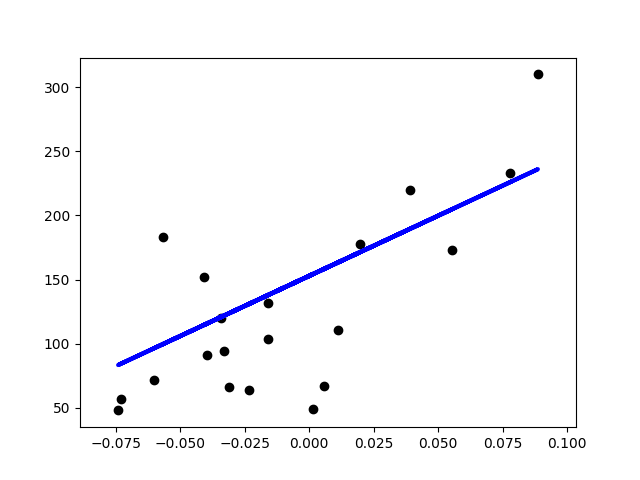
\includegraphics[scale=0.6]{../figures/Figure1.png}%
\linebreak%
\caption{This is a plot of the linear reg output. This plot was saved to a random directory and copied to the 'figures' folder of this report.}
\end{figure}
\\    
\begin{tabular}{llr}
\toprule
{} &             Results &  Values \\
\midrule
0 &      Coefficient(s) &     938 \\
1 &  Mean Squared Error &    2548 \\
2 &      Variance Score &       0 \\
\bottomrule
\end{tabular}
\\\caption{Results of the Logisitic Regression}


\lipsum[5]
